\section{Posters}
\begin{abstract_online}{Automatic Electronic Thesis and Dissertation Guideline Verification For Consistently Formatted Manuscripts}{%
    \underline{Mubanga C. Chibesa}$^{1}$, Albertina Mooka$^{1}$, Gift Muwele$^{1}$, Lwiime Shansonga$^{1}$, Lighton Phiri$^{1}$}{%
    }{%
    $^1$ The University Of Zambia}

Abstract:

Higher Education Institutions worldwide enforce guidelines and academic approaches to ensure scholarly integrity and adherence to academic standards(Razı et al., 2019).The University of Zambia, is not an exception. Just like most HEIs it offers  training to postgraduate students and one of the key aspects of postgraduate training is producing an Electronic Thesis and Dissertation manuscript The Directorate of Research and Graduate Studies (DRGS) provides guidelines which stipulate how ETD’s should be formatted. Successful graduation is dependent on postgraduate students’ manuscripts of which their conformance to the guidelines is a key aspect. Examiners and other relevant authorities are expected to verify and check if postgraduate students' manuscripts conform to the guidelines.
However, the process of  checking for conformance is a manual and tedious procedure, resulting in submission of inconsistently formatted manuscripts. Although this research seeks to ascertain the exact reasons why this is so, it is apparent that the primary task for the examiners is approving the content written in these manuscripts, and the secondary task being making sure that each and every manuscript is in conformance to the postgraduate guidelines and this is arguably an intense exercise. To address this challenge our  project seeks to implement a tool that will automate the process of checking ETD’s compliance against established postgraduate guidelines. The tool will leverage data mining techniques to perform these tasks. More specifically, document layout analysis (DLA)(Binmakhashen \& Mahmoud, 2019). The tool will flag off portions of ETD manuscripts that do not  conform to established guidelines. Hence, this will help resolve the inconsistencies in the format of submitted manuscripts. 

Methodology:

We will employ a mixed method approach  combining both qualitative and quantitative methods for data collection and analysis. Primary data is being collected through structured interviews and questionnaires, while secondary data involves  document analysis of postgraduate guidelines and archived historical ETDs. Convenient  sampling and purposive sampling  will be used to select participants, the selection is based on judgement and their willingness to participate in the study. The study is targeted on postgraduate examiners, alumni and current postgraduate students. Document analysis will be employed to understand the postgraduate guidelines stipulated in the (The University of Zambia, 2015) document and the identified guidelines are to be categorised into themes and a checklist will be prepared which will be used as a measurement instrument and each guideline, will be set as a question  and each question will be given a measurement scale of 1-5; content analysis will be used on randomly sampled ETDs in order to experimentally determine the extent of the problem using Park’s metrics of metadata quality (accuracy, consistency and completeness) and, finally, a DLA Natural Language Processing model will be implemented and will be evaluated using standard DLA metrics such as Structure Similarity Index and Intersection over Union.
This DLA pipeline is  hinged on Artificial intelligence and Natural language processing(NLP)(Mishra \& Kumar, 2020). We also  leveraged  an open source package called Deepdoctetion for the implementation of the software tool. 
For the development process, Agile methodologies, specifically scrum, will be used for software development, with document layout techniques applied to enhance the Deepdoctetion package in the process. We also accessed the accuracy and usability of the tool through a benchmark dataset composed of historical ETDs archived on The University of Zambia institutional repository. Measurement instruments include structured interview guides and a checklist to evaluate the threshold of compliance of historical ETDs.
Preliminary Findings  and Discussion
Empirical Analysis of Historical Archived ETDs
The analysis of historical archived manuscripts against postgraduate guidelines revealed that most manuscripts did not adhere to the guidelines. The preliminary findings indicate that the majority of the students from all the schools at the institution performed poorly on sections such as the copyright declaration page which had the lowest compliance, with much lower scores in accuracy (2.227), consistency (2.194), and completeness (2.037). This suggests that this section of the manuscripts frequently falls short of meeting the required standards, highlighting a critical area for improvement. This is followed by the declaration page with the second lowest scores in accuracy (3.042), consistency (2.681) and completeness (2.835). The compliance to miscellaneous requirements also had some low scores in accuracy (3.774), consistency (3.760) and completeness (3.841).
Overall middle-ranking sections include the title Page with the following compliance scores in accuracy (4.078), consistency (3.861) and completeness (4.023).  Whereas compliance on the certificate of approval indicates the following scores in accuracy (4.293),consistency (4.304) and completeness (4.322). Similarly, the end matter section with the following compliance scores in accuracy (4.581), consistency (4.471) and completeness (4.551).Lastly, compliance to pagination had the following scores in accuracy (4.634), consistency (4.629) and completeness (4.623). 
However, while these sections generally show good compliance, the moderate degree of variation suggests that there are some inconsistencies in adherence to the guidelines, and targeted improvements could enhance their overall performance.
Overall, the "Order Of Text" demonstrates exceptional compliance with nearly perfect scores in accuracy (4.969), consistency (5) and completeness (5). Similarly, compliance to the prescribed length of an ETD indicates remarkable scores in accuracy (5), consistency (5) and completeness (5).
Survey responses for current postgraduate students
According to the responses from current postgraduate students, the most common challenges in ensuring correct document formatting in accordance with the universities guidelines included difficulties with citation management, generating the correct table of contents, and formatting tables and figures. Out of 22 respondents, seven (7) highlighted that they find difficulties in adjusting their manuscripts to  the prescribed margins, another seven (7) highlighted difficulties when working on tables and figures. Ten respondents stated that the most challenging aspect is with regards to generating references and citations. Five respondents also highlighted that following the prescribed table of contents is challenging for them.
Of the 22 respondents, 50\% stated that they were not very familiar with the postgraduate guidelines of the institution while 6 % stated that they were somewhat familiar with the guidelines. Of the remaining 8%, 4% stated that they were very familiar with the guidelines while the other 4% stated that they were not familiar with the guidelines at all.

Survey results indicate that postgraduate alumni faced challenges with formatting their manuscripts, particularly in adding tables, maps, figures (5 respondents), managing citations (4 respondents), and inserting footnotes (2 respondents). These difficulties align with the low scoring of miscellaneous guidelines (covering citations, figures, and tables) in historical ETD analyses.

Examiners also reported challenges in manually verifying manuscript compliance. With a high student-to-examiner ratio in some schools, the workload can be overwhelming, limiting their ability to be thorough. Due to time constraints, examiners often review up to 50 manuscripts per sitting to provide timely feedback and avoid delaying student research. Furthermore, examiners stated that they find themselves either resending the guidelines to the students or scheduling short seminars mid-research to re-educate the students about the guidelines when they notice a lot of inconsistencies in the  submitted manuscripts.
Conclusion
The use of DLA methods to create a pipeline that will curtail the challenge of ensuring and checking compliance of ETDs to postgraduate guidelines at the university of Zambia has proven to be the most efficient solution. The development of an ETD automatic guideline verification tool presents an opportunity to enhance efficiency as well as promote consistency in the quality of ETDs while alleviating the challenges faced in the process of manually checking for compliance consequently reducing the workload for students, supervisors and examiners alike. 

References:

Mishra, B. K., \& Kumar, R. (2020). Natural Language Processing in Artificial Intelligence.
Razı, S., Glendinning, I., \& Foltýnek, T. (2019). Towards Consistency and Transparency in Academic Integrity. Peter Lang Gmbh, Internationaler Verlag Der Wissenschaften.
Binmakhashen, G. M., \& Mahmoud, S. A. (2019). Document Layout Analysis: A Comprehensive Survey. ACM Comput. Surv., 52(6), 1–36.
The University of Zambia. (2015). Directorate of Research and Graduate Studies: Postgraduate regulations.

\begin{center}
    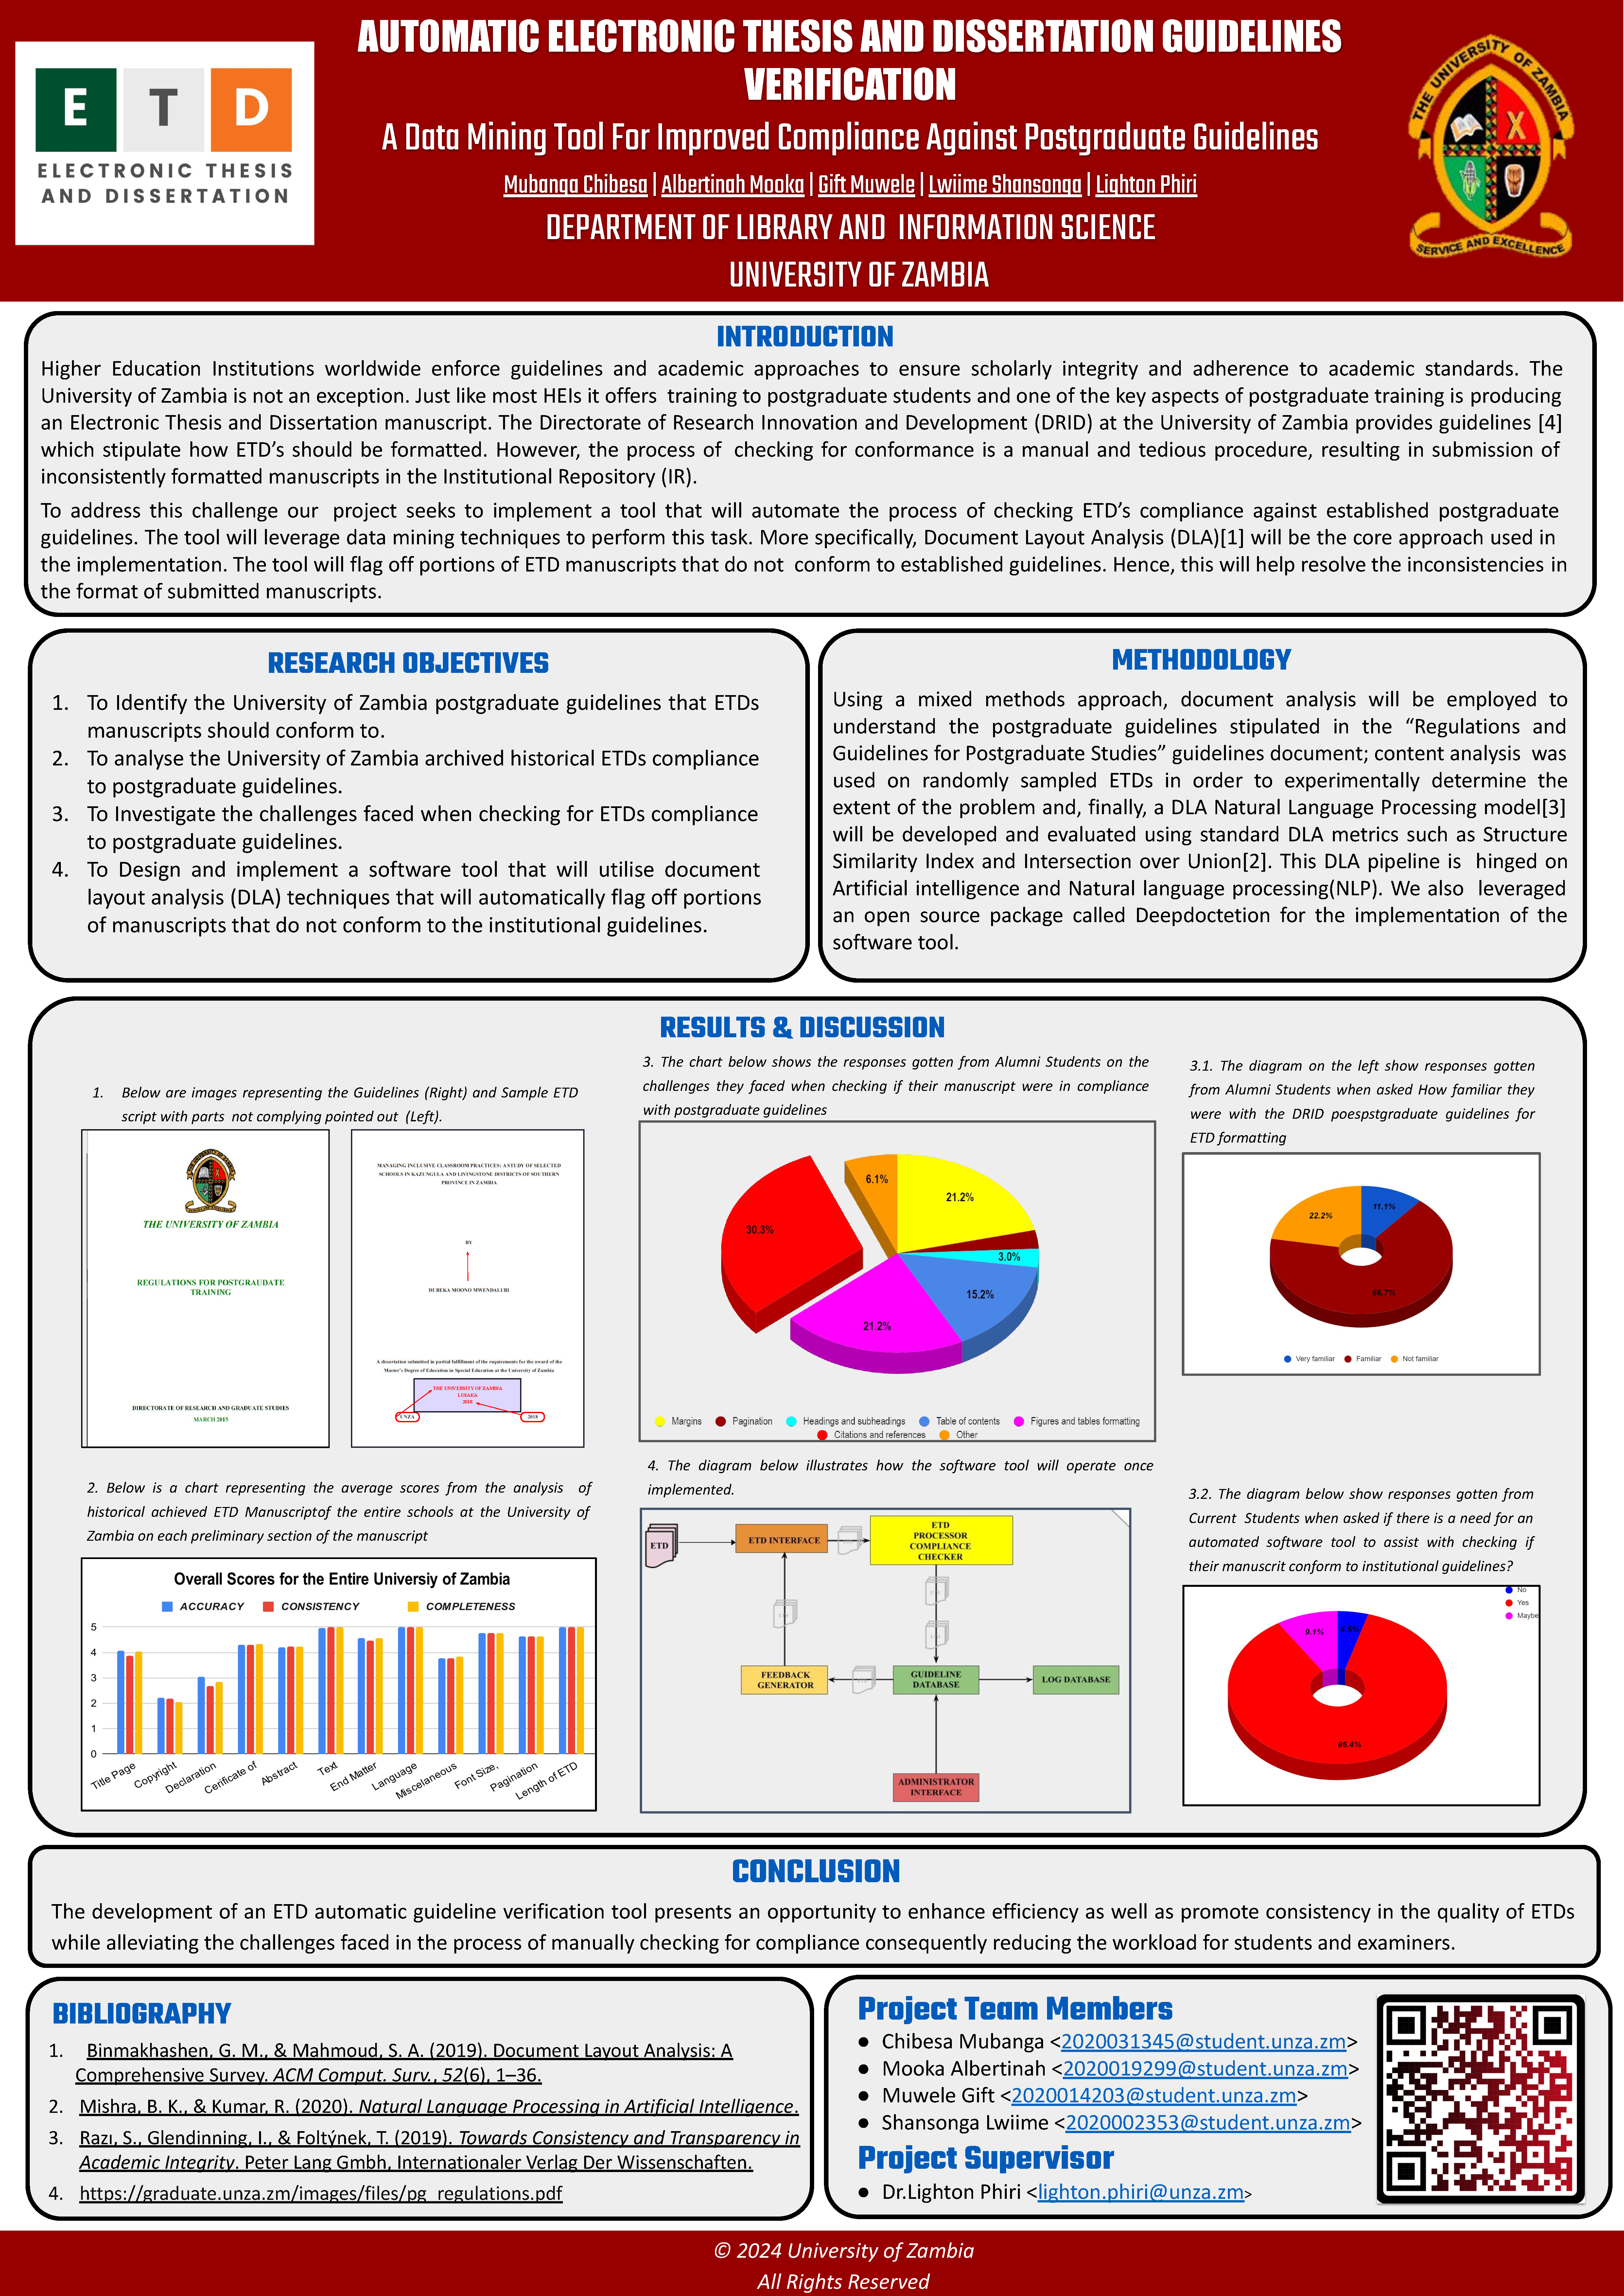
\includepdf[pages=1, width=\linewidth]{./conference_assets/docs-poster-etd24-46}
\end{center}

\end{abstract_online}
